\section{Oracle UCM}

\subsection{Allgemein}
Oracle Universal Content Management basiert auf der Software Stellent von der gleichnamigen Firma Stellent, welche im November 2006\footnote{Quelle: \cite{OraPress}} von Oracle gekauft / erworben wurde.





\begin{center}
Bild \cite{Huff06} S 17
\end{center}

Sessionanzahl

Für was wird sie im FZK benutzt, auch Windows nennen

\subsection{Aufbau / Architektur}

Die Architektur des Oracle UCM Systems gliedert sich in separate Komponenten auf wie in Abbildung \ref{ucm-arch} gezeigt.

\begin{figure}[ht]
	\centering
	   \fbox{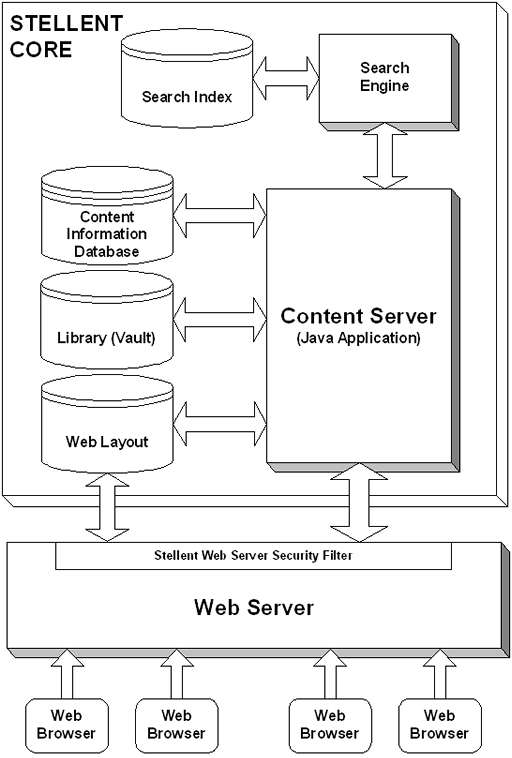
\includegraphics[width=0.5\textwidth]{bilder/basic_architecture.png}}
		\caption[Oracle UCM Architektur]{Oracle UCM Architektur\protect\footnote}
		\label{ucm-arch}
\end{figure}
\footnotetext{Quelle: \url{http://www.club-oracle.com/forums/oracle-universal-content-management-ucm-aka-stellent-t146/}}


\subsubsection{Content Server}
\subsubsection{Vault und Web Layout}
\subsubsection{Inbound Refinery}
\subsubsection{Search Engine}
\subsubsection{Webserver}

Oracle DB als Grundlage

FZK Bilddatenbank erwähnen


Einchecken -> Konvertieren -> Indexieren
\subsection{Überwachungselemente}
Die Überwachung einer Dienstes über ein Netzwerk verteilt sich auf verschiedenen Ebenen mit unterschiedlichen Gewichtungen.
Zum Beispiel stellt das simple Senden eines Pings an den entsprechenden Server die niedrigste und primitivste Stufe dar, da hier lediglich die Netzwerkschnittstelle des Servers auf ihre Funktionalität und dabei der Status der Netzwerkstrecke getestet wird.(Rechner an und Netzwerk ok)
Ob die Anwendung überhaupt auf dem Server läuft und wenn, in welchem Zustand sie sich befindet (betriebsfähig, reagiert nicht mehr usw.), muss auf eine andere Weise herausgefunden werden.

Dabei lässt sich aus den verschiedenen Überwachungselemente folgende drei Kategorien bilden/ableiten:

\subsubsection{Statusabfragen}
Diese Kategorie besteht aus einfacheren Überprüfungen, die jeweils den Status des Überwachungselementes überwachen.
Dabei können weitere Untergruppen gebildet werden.

(Irgendwie Hierarchie verdeutlichen: zuerst ping als Grundlage, dann prozesse und services dann funktionschecks, bloss wie? Visio Bild?)

\paragraph{System}
\begin{itemize}
\item \textbf{Ping} Überprüft, ob der Rechner vom Nagios-Server über das Netzwerk erreichbar ist.
\item \textbf{Prozessorauslastung} Überwacht die Auslastung des Prozessors und schlägt bei ungewöhnlich hohen Werten Alarm.
\item \textbf{Festplattenspeicherausnutzung} Überwacht die Speicherplatzauslastungen der verschiedenen Festplattenpartitionen, damit immer genügend Speicherplatz für Anwendungen und Betriebssystem verfügbar ist.
\item Temperatur ??? Die ganzen Standardüberwachungen -> Thüllmann
\item \textbf{Sessionanzahl} Anzahl der am CMS angemeldeten Benutzer, da aus Performanzgründen eine Obergrenze mit einer maximalen Anzahl festgelegt ist.
\end{itemize}

\paragraph{Prozesse}
\begin{itemize}
\item \textbf{IdcServerNT.exe} Der Windowsprozess des Stellent-Servers
\item \textbf{IdcAdminNT.exe} Der Windowsprozess für die Administration (Webinterface?) des Stellent-Servers
\item \textbf{w3wp.exe} Der Windowsprozess des Microsoft "`Internet Information Services"'
\end{itemize}

\paragraph{Services}
\begin{itemize}
\item \textbf{IdcContentService???}  Den Zustand des "`Content-Dienstes"'-\pictext{sccdms01} überprüfen.
\item \textbf{IdcAdminService???}  Den Zustand des "`Administrations-Dienstes"'-\pictext{sccdms01\_admin} überprüfen.
\item \textbf{Zeitsynchronisationsdienst:} Überprüfen, ob der \pictext{W32TIME}-Dienst, der für den Zeitabgleich mit einem Zeitserver zuständig ist, läuft und die Abweichung zwischen Client und Zeitserver festhalten.
\item \textbf{Antivirusdienst}: Den Zustand den Dienstes überprüfen, der für die ständig Updates des Virusscanners Symantec AntiVirus notwendig ist.
\end{itemize}

\subsubsection{Überwachung der Funktionalität}
Durch die vorherigen Tests kann herausgefunden werden, ob eine Anwendung oder ein Dienst auf dem Server gestarten wurde.
Die Funktionalität kann durch solche Überprüfungen jedoch \textbf{nicht} sichergestellt werden.
Da beispielsweise der Prozess bzw. Dienst des Webservers gestartet ist, jedoch keine Webseite aufgerufen werden kann.
%Da beispielsweise der Webserver aufgrund eines kritischen Fehlers nicht erreichbar ist, der Prozess bzw. Dienst dennoch läuft.
Daher muss eine weitere Art von Überprüfungen/Checks die Anwendungen auf ihre Funktionalität (hin) überprüfen.

\begin{itemize}
\item \textbf{Webserver} Aufruf einer Webseite auf dem Server. Wenn auf diese Anfrage eine gültige Antwort in Form einer Statuscode-Meldung erfolgt, kann der reale/wirkliche Zustand des Webservers festgestellt werden.

\item \textbf{Webinterface des Oracle UCM} Zusätzlich wird mit dieser Abfrage die Integration des Conten-Management-Systems in den Webserver überwacht, da hier nicht nur der Webserver, sondern eine UCM spezifische Webseite abgefragt wird.

\item \textbf{Benutzeranmeldung am Oracle UCM} Hier wird getesten, ob sich ein Benutzer erfolgreich am System anmelden kann.
Dies wird mit Anmeldungsdaten eines lokalen Benutzers und eines Active Directory-Benutzers durchgeführt um gleichzeitig/zusätzlich die Verbindung zum ADS-Server zu testen.

\item \textbf{Oracle Datenbank} Wenn keine Verbindung zur Oracle Datenbank möglich ist, können keine neuen Informationen gespeichert werden. 
(zitat riester: läuft das system noch pseudomäßig, wirft aber jede Menge Fehler)

\item \textbf{Status von Cronjobs} In periodischen Zeitabständen werden Programme aufgerufen, deren Aufruf und Endstatus/Endergebniss überwacht werden muss. 
Damit nicht das vorherige Ergebnis zu einem False Negative führt, müssen hier zusätzliche Zeitinformationen/zeitliche Parameter beachtet/bedacht werden.

\item \textbf{Einchecken von Dokumenten} Damit die eigentliche Aufgabe des Dokumentenverwaltungssystem überwacht werden kann, werden verschiedene Datenformate testweise eingecheckt. 
Dabei wird die Antwort der Anwendung auf das Hinzufügen der Dateien analysiert.

\item \textbf{Konvertierung} Da das hinzugefügte Dokument nicht nur einfach auf dem Server gespeichert wird, sondern dabei auch in ein anderes Format umgewandelt wird, muss diese Konvertierung zusätzlich überwacht werden. 
Wird beispielsweise ein Bild eingecheckt, wird dieses mehrfach in verschiedenen Auflösung oder als anderes Bilddateiformat gespeichert. 
Ob diese Transformation erfolgreich ablief, kann anhand dieser neuen Dateien festgestellt werden.

\item \textbf{Indizierung} Bei dem Einchecken sollen auch gleichzeitig zusätzliche Informationen über das Dokument festgehalten werden. 
Diese Informationen können beispielsweise der Name des Authors, das Erstellungsdatum der Datei oder - bei Bildern - der verwendete Farbraum sein. 
Bei der Suche nach einem Dokument können diese Informationen als zusätzliche Suchkriterien verwendet werden.
Daher müss überprüft werden, ob diese Daten richtig ausgelesen werden, der Datenbank hinzugefügt und vom Anwender abgefragt werden können. Dabei werden auch zuvor festgelegte/ausgewählte Testdateien verwendet.

\item \textbf{Suchfunktion} Nach einer erfolgreichen Indizierung muss das eingecheckte Dokument per Suchanfrage gefunden werden.
Ob die Suche und Indizierung erfolgreich abgelaufen ist, wird zusätzlich überprüft. 

\item Benutzersimulation!

\end{itemize}

\subsubsection{Auswerten von Logdateien}
Die zwei bisherigen Kategorien beinhalten simple Zustandsüberprüfungen oder aktive Funktionaltests.
In dieser Kategorie werden zusätzlich verschiedene Logs auf spezielle Warnungs- und Fehlermeldungen anhand entsprechender eindeutigen Signal/Stopwörter untersucht.
Dies ist notwendig um Fehlverhalten der Anwendung zu erkennen, das nicht mit den vorherigen Überwachungselementen entdeckt wurde.
Desweiteren können durch die Analyse der Logdateien etwaige Alarmmeldungen der bisherigen Tests bestätigt, begründet oder aufgehoben werden.
Somit bietet das Auswerten der Logdateien zusätzliche Sicherheit False Positive- oder False Negative-Meldungen auszuschliessen.

Die Oracle UCM Anwendung erstellt drei verschiedene Arten von Logdateien:\footnote{Quelle: \cite{UCMlog09}}

\begin{itemize}
\item \textbf{Content Server Log} 
\item \textbf{Inbound Refinery Log}
\item \textbf{Archiver Log}
\end{itemize}

Um alle Logs ohne Probleme im Internetbrowser anzuzeigen, liegen alle Logdateien im HTML-Format vor.
Alle drei Arten von Logs bestehen jeweils aus 30 verschiedenen Dateien, die sich täglich abwechseln.
Dadruch wird für jeden Tag im Monat eine separate Datei angelegt, um bei vielen Warnungs- und Fehlermeldungen durch die chronologische Anordnung/Hierarchie den Überblick zu behalten.
So werden die Logdateien zwangsweise nach 30 Tagen nacheinander überschrieben.

Diese Rotation der Logdateien muss bei der Durchsuchung nach Signal/Stopwörter beachtet werden, damit stets die aktuelle Logdatei überwacht wird und keine veralteten Informationen für False Positives-Meldungen durch Nagios sorgen.

%wieso nur plugin check\_log und nicht einfahc umfangreicheres Standalone Programmw ie syslog\_nd oder 8pussy


Übersichttabelle? wie mit beschreibung verbinden?











